
\documentclass[12pt,a4paper]{article}
\usepackage[utf8]{inputenc}
\usepackage[russian]{babel}
\usepackage{amsmath}
\usepackage{amsfonts}
\usepackage{amssymb}
\usepackage{graphicx}
\usepackage{float}
\usepackage{listings}
\usepackage[left=2cm,right=2cm,top=2cm,bottom=2cm]{geometry}
\usepackage{tocloft}
\usepackage{placeins}

\usepackage{titlesec}
\usepackage{hyperref}

% section and subsection formmatting
\titleformat{\section}[block]{\normalfont\Large\bfseries\filcenter}{\thesection}{1em}{}
\titleformat{\subsection}{\normalfont\large\bfseries}{\thesubsection}{1em}{}

% Customize the table of contents to GOST standards
\renewcommand{\cftsecdotsep}{\cftdotsep}
\renewcommand{\cftsecfont}{\normalfont}
\renewcommand{\cftsecpagefont}{\normalfont}
\renewcommand{\cftsecpresnum}{\S\ }
\newlength{\stdindent}
\setlength{\stdindent}{\cftsecnumwidth}
\addtolength{\cftsecnumwidth}{3mm}

\numberwithin{subsection}{section}
\usepackage{xcolor}
\lstset{
basicstyle=\ttfamily,
columns=fullflexible,
frame=single,
breaklines=true,
postbreak=\mbox{\textcolor{red}{$\hookrightarrow$}\space},
keywordstyle=\color{blue},
commentstyle=\color{green},
}


\begin{document}

\begin{titlepage}
    \begin{center}
        \vspace*{2cm}
        {\Large \textbf{МИНИСТЕРСТВО НАУКИ И ВЫСШЕГО ОБРАЗОВАНИЯ РОССИЙСКОЙ ФЕДЕРАЦИИ}}\\
        \vspace{0.5cm}
        {\Large \textbf{ФЕДЕРАЛЬНОЕ ГОСУДАРСТВЕННОЕ АВТОНОМНОЕ ОБРАЗОВАТЕЛЬНОЕ УЧРЕЖДЕНИЕ ВЫСШЕГО ОБРАЗОВАНИЯ}}\\
        \vspace{0.5cm}
        {\Large \textbf{НОВОСИБИРСКИЙ НАЦИОНАЛЬНЫЙ ИССЛЕДОВАТЕЛЬСКИЙ ГОСУДАРСТВЕННЫЙ УНИВЕРСИТЕТ}}\\
        \vspace{0.5cm}
        {\large \textbf{Факультет информационных технологий}}\\
        \vspace{0.5cm}
        {\large \textbf{Кафедра параллельных вычислений}}\\
        \vspace{1cm}
         {\Large \textbf{ОТЧЕТ О ВЫПОЛНЕНИИ ПРАКТИЧЕСКОЙ РАБОТЫ}}
        \vspace{0.5cm}
        
        {\Large \textbf{Практическая работа №1}}\\
        \vspace{0.5cm}
         {\large Определение времени работы прикладных программ}\\
        \vspace{0.5cm}
        {\large студента 2 курса, группы 23201}\\
        \vspace{0.5cm}
        {\Large \textbf{Сорокина Матвея Павловича}}\\
        \vspace{1cm}
        {\large Направление 09.03.01 -- ''Информатика и вычислительная техника''}\\
        \vspace{2cm}
        
        \begin{flushright}
            \textbf{Преподаватель: А.С. Матвеев} \\
        \end{flushright}
        
        \vfill
        
        {\large Новосибирск, 2024 г.}
    \end{center}
\end{titlepage}

\tableofcontents

\newpage

\setcounter{page}{2}


\section{ЦЕЛЬ}
Изучение методов измерения времени работы программы, 
оптимизации этих измерений, анализ влияния различных 
уровней оптимизации компилятора GCC на время 
выполнения программы.

\section{ЗАДАНИЕ}
В ходе работы было необходимо выполнить следующие задачи:
\begin{itemize}
    \item Написать программу на языке C или C++, которая реализует выбранный алгоритм из задания.
    \item Проверить правильность работы программы на нескольких тестовых наборах входных данных.
    \item Выбрать значение параметра N таким, чтобы время работы программы было порядка 15 секунд.
    \item По приведенной методике определить время работы подпрограммы тестовой программы с 
    относительной погрешностью не более 1\%.
    \item Составить отчет по лабораторной работе.
\end{itemize}

\newpage


\section{ОПИСАНИЕ РАБОТЫ}

%\setcounter{subsection}{0}
%\renewcommand{\thesubsection}{1.\arabic{subsection}}
% \subsection{}
\begin{itemize}
    \item Реализовано задание №4 - алгоритм вычисления синуса с помощью разложения 
    в степенной ряд по превым \textit{N} членам данного ряда на языке \textit{C++}.
    \item Для измерения времени работы программы использовалась библиотечная 
    функция \textit{clock\_gettime}
    из библиотеки \textit{time.h}.
    \\
    \\
    Код программы также предоставлен (см. \hyperref[app:listing]{Приложение 1}), 
    также предоставлен \textit{bash-скрипт}, компилирующий и запускающий программу 
    с конкретными знаениями x и N, записывающий время вычисления синуса угла с 
    различными уровнями оптимизации компилятора \textit{GCC} в \textit{report.csv} 
    файл (см. \hyperref[app:listing]{Приложение 2}), после чего запускает
    \textit{create\_table.sh}, визуализирующий информацию из report.csv.
    \\
    \\
    Время замерялось перед началом и после окончания работы функции, вычисляющей
    синус заданного угла. Разность этих двух значений дает общее время выполнения функции. 
    Для проверки точности измерений, код программы запускается несколько раз.
\end{itemize}


\section{ЗАКЛЮЧЕНИЕ}
В ходе данной лабораторной работы мы познакомились с различными методами измерения 
работы программ и научились пользоваться ими на практике.

\newpage


\section*{Приложения}\label{app:listing}
%\addcontentsline{toc}{section}{Приложение}
%\setcounter{subsection}{0}
%\renewcommand{\thesubsection}{2.\arabic{subsection}}

\subsection*{Приложение 1: Исходный код программы}
\begin{lstlisting}
    #include <iostream>
    #include <time.h>
    #include <cstdlib> // for atoi and atof
    #include <cmath> // for pow
    
    long double DegToRad(long double deg) {
        return deg * M_PI / 180;
    }
    
    long double SinCalculation(long double x, long long n) {
        long double sin = 0;
        long double prev = x;
        long double sign = 1.0;
    
        for (long long i = 1; i < n; i++) {
            sin += sign * prev;
            prev *= (x * x) / ((2 * i) * (2 * i + 1));
            sign = -sign;
        }
    
        return sin;
    }
    
    int main(int argc, char *argv[]) {
        if (argc != 3) {
            std::cerr << "Usage: <angle in degrees> <number of terms>" << std::endl;
            return 0;
        }
    
        struct timespec start, end;
        long double x = atoll(argv[1]);
        long long n = atoll(argv[2]);
    
        std::cout << "x = " << x << ", n = " << n << std::endl;
    
        int runs = 5;
        double time_total = 0;
    
        for (long long i = 0; i < runs; i++) {
            clock_gettime(CLOCK_MONOTONIC_RAW, &start);
            double rad_x = DegToRad(x);
            long double sin = SinCalculation(rad_x, n);
            clock_gettime(CLOCK_MONOTONIC_RAW, &end);
    
            double taken_time = (end.tv_sec - start.tv_sec) + (end.tv_nsec - start.tv_nsec) / 1e9;
            std::cout << "sin(" << x << ") = " << sin << std::endl;
            std::cout << "Run " << i + 1 << " took " << taken_time << " seconds to complete" << "\n" << std::endl;
            time_total += taken_time;
        }
    
        std::cout << "Average time: " << time_total / runs << " seconds" << std::endl;
        return 0;
    }
    
\end{lstlisting}

\subsection*{Приложение 2: bash-скрипт для компиляции и запуска программы 
\textit{SinCalculation.cpp}, записи результата в файл report.csv}

\begin{lstlisting}
#!/bin/bash

input="SinCalculation.cpp"

optimization_levels=("-O0" "-O1" "-O2" "-O3" "-Os")
n=2300000000
x=90

echo "Optimixation level, N value, X value, Time taken (seconds)" > report.csv

for i in "${optimization_levels[@]}"; do
    g++ -o sin $input $i -std=c++11
    output=$(./sin $x $n | grep "Average time:" | awk '{print $3}')
    echo "$i, $n, $x, $output" >> report.csv
done

echo "Successfully generated report.csv"

./create_table.sh    
\end{lstlisting}

\newpage


\subsection*{Приложение 3: результат работы \textit{bash-скрипта}
\textit{compile\_and\_run.sh}}

\begin{figure}[H]
    % \centering
    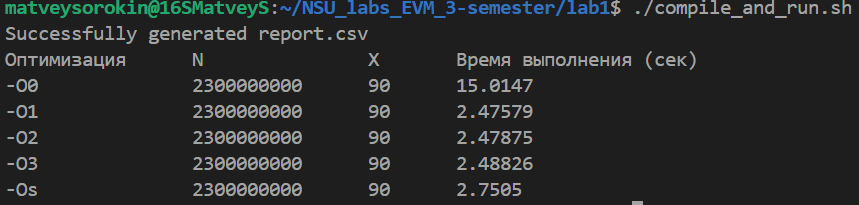
\includegraphics[width=0.8\textwidth]{3.png}
\end{figure}

\vspace{1cm}


\subsection*{Приложение 4: результаты измерений в \textit{report.csv} с использованием 
\textit{bash-скрипта} \textit{compile\_and\_run.sh}}

\begin{figure}[H]
    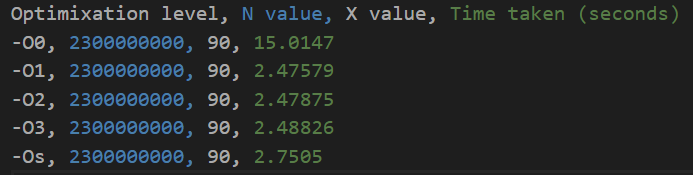
\includegraphics[width=0.8\textwidth]{4.png}
\end{figure}

\vspace{1cm}


\subsection*{Приложение 5: результат работы скомпилированной программы 
\textit{SinCalculation.cpp}}

\begin{figure}[H]
    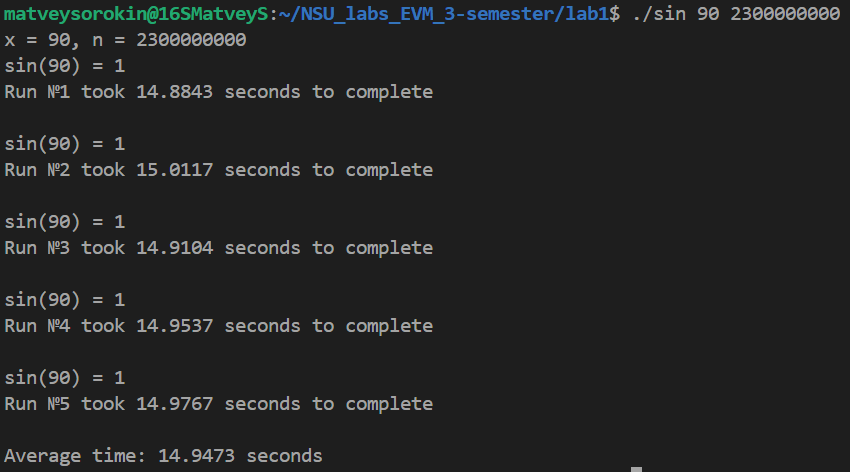
\includegraphics[width=0.8\textwidth]{5.png}
\end{figure}


\end{document}
